\documentclass[11pt,a4paper]{article}

\usepackage[margin=1in]{geometry}
\usepackage{times}
\usepackage{microtype}
\usepackage{amsmath,amssymb,amsfonts,amsthm}
\usepackage{booktabs}
\usepackage{multirow}
\usepackage{adjustbox}
\usepackage{enumitem}
\usepackage{algorithm}
\usepackage{algorithmic}
\usepackage{graphicx}
\usepackage{subcaption}
\usepackage{float}
\usepackage{url}
\usepackage[colorlinks=true,linkcolor=blue,citecolor=blue,urlcolor=blue]{hyperref}

\newtheorem{definition}{Definition}
\newtheorem{theorem}{Theorem}
\newtheorem{corollary}{Corollary}

\newcommand{\D}{\mathcal{D}}
\newcommand{\I}{\mathcal{I}}
\newcommand{\GammaSet}{\Gamma}
\newcommand{\supp}{\operatorname{sup}}
\newcommand{\cl}{\operatorname{cl}}
\newcommand{\aocc}{\operatorname{aocc}}
\newcommand{\CHUOI}{\operatorname{CHUOI}}
\newcommand{\HUOI}{\operatorname{HUOI}}
\newcommand{\RUU}{\operatorname{RUU}}
\newcommand{\OUB}{\operatorname{OUB}}

\title{\textbf{CHUO-Miner: Closed High-Utility Occupancy Itemset Mining with Lossless Hybrid Signatures}}

\author{
Quan Van\\
Independent Researcher\\
\texttt{vanhaminhquan2406@gmail.com}
}

\date{}

\begin{document}
\maketitle

\begin{abstract}
High-utility itemset mining discovers profitable patterns, closed high-utility itemset mining compresses redundant high-utility outputs, and high-occupancy itemset mining captures patterns that dominate the transactions in which they appear. These objectives have usually been studied separately. This paper studies \emph{Closed High-Utility Occupancy Itemset Mining} (CHUOIM), where a valid pattern must simultaneously satisfy minimum support, minimum absolute utility, minimum classical average occupancy, and support-closure. We introduce CHUO-Miner, a vertical COU-list algorithm that combines exact utility accounting, reciprocal transaction-length occupancy accounting, remaining-utility pruning, an occupancy-envelope upper bound, backward closure pruning, forward closure jumping, and lossless CHUO-signatures. Experiments on Foodmart, Liquor, and Chainstore show that CHUO-Miner produces compact closed hybrid representatives across diverse thresholds. Compared with EFIM, CHUI-Miner, and EFIM-Closed, it reduces output size by orders of magnitude and avoids timeouts on Chainstore. Compared with MHOUI, it is slower but solves a stricter problem by returning support-closed representatives with reconstructable support-equivalent subpatterns.
\end{abstract}

\noindent\textbf{Keywords:}
high-utility itemset mining; closed itemset mining; occupancy mining; utility occupancy; CHUI; HUIM; compact pattern representation.

\section{Introduction}

High-utility itemset mining (HUIM) focuses on absolute utility and is effective for discovering profitable itemsets. Algorithms such as Two-Phase, HUI-Miner, FHM, and EFIM introduced transaction-weighted utilization, utility-lists, co-occurrence pruning, projection, and transaction merging to make this task practical \cite{Liu2005TwoPhase,Liu2012HUIMiner,FournierViger2014FHM,Zida2017EFIM}. A separate line of work studies closed high-utility itemsets (CHUIs), where closed representatives compactly describe support-equivalent utility patterns \cite{Wu2015CHUIMiner}. Occupancy mining asks whether a pattern occupies a large fraction of the transactions in which it occurs \cite{Deng2020HOI}. Related utility-occupancy work such as HUOPM uses the ratio between itemset utility and transaction utility, which is different from classical item-count occupancy \cite{Gan2020HUOPM}.

These families leave a hybrid gap. A profitable pattern may occupy only a tiny structural portion of each basket. A high-occupancy pattern may be unprofitable. A closed high-utility pattern may still ignore occupancy. A utility-occupancy pattern may optimize a ratio but not absolute profit. This paper formalizes a stricter mining target: itemsets that are high utility, high classical occupancy, and support-closed.

The contribution is threefold:
\begin{itemize}
    \item We define Closed High-Utility Occupancy Itemsets (CHUOIs) using support, absolute utility, classical average occupancy, and support-closure.
    \item We show that within a support-equivalence class, the closure is the Pareto-maximum representative for both utility and classical occupancy under positive utilities.
    \item We implement and evaluate CHUO-Miner, a vertical algorithm with COU-lists, remaining-utility pruning, occupancy-envelope pruning, closure jumping, closure hashing, and CHUO-signature reconstruction.
\end{itemize}

\section{Problem Formulation}

Let \(\D=\{T_1,\ldots,T_n\}\) be a positive-utility transaction database over item universe \(\I\). Each item \(i\in T_q\) has positive utility \(u(i,T_q)\). For an itemset \(X\), define
\[
\GammaSet(X)=\{T_q\in \D\mid X\subseteq T_q\},
\qquad
\supp(X)=|\GammaSet(X)|.
\]
The utility of \(X\) is
\[
u(X)=\sum_{T_q\in\GammaSet(X)}\sum_{i\in X}u(i,T_q).
\]
Unlike HUOPM-style utility occupancy, CHUOIM uses classical item-count occupancy:
\[
\aocc(X)=
\frac{1}{\supp(X)}
\sum_{T_q\in\GammaSet(X)}
\frac{|X|}{|T_q|}.
\]

\begin{definition}[High-Utility Occupancy Itemset]
Given minimum support \(\sigma\), minimum utility \(\mu\), and minimum occupancy \(\beta\), an itemset \(X\neq\emptyset\) is a high-utility occupancy itemset if
\[
\supp(X)\ge\sigma,\qquad u(X)\ge\mu,\qquad \aocc(X)\ge\beta.
\]
The set of all such itemsets is denoted \(\HUOI(\D,\sigma,\mu,\beta)\).
\end{definition}

Support-equivalence is defined by identical supporting transaction sets:
\[
X\equiv Y \iff \GammaSet(X)=\GammaSet(Y).
\]
The support-closure of \(X\) is
\[
\cl(X)=\bigcap_{T\in\GammaSet(X)}T.
\]

\begin{definition}[Closed High-Utility Occupancy Itemset]
An itemset \(X\) is a CHUOI if
\[
X\in \HUOI(\D,\sigma,\mu,\beta)
\quad\text{and}\quad
\cl(X)=X.
\]
\end{definition}

\begin{theorem}[Closure Maximizes the Hybrid Profile]
For any itemset \(X\), let \(C=\cl(X)\). Under positive utilities,
\[
\supp(C)=\supp(X),\qquad u(C)\ge u(X),\qquad \aocc(C)\ge\aocc(X).
\]
If \(C\neq X\), the utility and occupancy inequalities are strict.
\end{theorem}

\begin{proof}
Closure preserves the supporting transaction set, hence support is unchanged. Since \(C\supseteq X\), every supporting transaction contributes all items in \(X\) plus positive-utility items from \(C\setminus X\), so \(u(C)\ge u(X)\). The occupancy denominator \(|T_q|\) is unchanged while the numerator increases from \(|X|\) to \(|C|\), so \(\aocc(C)\ge\aocc(X)\). Strictness follows from positive utility and \(|C|>|X|\).
\end{proof}

\begin{corollary}[Lossless Closed Hybrid Representation]
Every feasible \(X\in\HUOI(\D,\sigma,\mu,\beta)\) maps to a unique closed representative \(C=\cl(X)\in\CHUOI(\D,\sigma,\mu,\beta)\).
\end{corollary}

For lossless reconstruction of support-equivalent subpatterns, CHUO-Miner stores a CHUO-signature for each emitted \(C\):
\[
\Pi(C)=\left(C,\supp(C),R_C,\{V_C(i)\}_{i\in C}\right),
\]
where
\[
R_C=\sum_{T\in\GammaSet(C)}\frac{1}{|T|},
\qquad
V_C(i)=\sum_{T\in\GammaSet(C)}u(i,T).
\]
For every \(A\subseteq C\) such that \(\cl(A)=C\),
\[
u(A)=\sum_{i\in A}V_C(i),
\qquad
\aocc(A)=\frac{|A|}{\supp(C)}R_C.
\]

\section{CHUO-Miner}

CHUO-Miner is a vertical depth-first miner. Its central structure is the COU-list. For a pattern \(X\), each supporting transaction contributes one entry:
\[
e=\langle tid,pos,iu,ru,rc,invlen\rangle,
\]
where \(iu=u(X,T)\), \(ru\) is the remaining utility after the last item position, \(rc\) is the remaining extension count, and \(invlen=1/|T|\). From a COU-list \(L_X\),
\[
\supp(X)=|L_X|,
\qquad
u(X)=\sum_{e\in L_X}e.iu,
\]
\[
\RUU(X)=\sum_{e\in L_X}(e.iu+e.ru),
\qquad
\aocc(X)=|X|\frac{\sum_{e\in L_X}e.invlen}{|L_X|}.
\]

\subsection{Pruning Bounds}

At the root, CHUO-Miner removes items with support below \(\sigma\) or TWU below \(\mu\). During search, two upper bounds are used.

\begin{theorem}[Remaining Utility Upper Bound]
For any descendant \(Y\supseteq X\),
\[
u(Y)\le \RUU(X).
\]
\end{theorem}

\begin{theorem}[Occupancy Envelope Upper Bound]
For each \(e\in L_X\), define
\[
\lambda_e=(|X|+e.rc)e.invlen.
\]
Let \(\lambda_{(1)}\ge\cdots\ge\lambda_{(|L_X|)}\). For every descendant \(Y\supseteq X\) with support at least \(\sigma\),
\[
\aocc(Y)\le \OUB(X)=\frac{1}{\sigma}\sum_{j=1}^{\sigma}\lambda_{(j)}.
\]
\end{theorem}

Thus a branch is pruned if either \(\RUU(X)<\mu\) or \(\OUB(X)<\beta\).

\subsection{Closure Handling}

Closure is support-based. CHUO-Miner materializes singleton TID bitsets and lazily materializes node bitsets. If a prior item \(z\) has
\[
\supp(X\cup\{z\})=\supp(X),
\]
then \(X\) has a backward extension and the subtree is pruned. If a suffix item has the same support as \(X\), CHUO-Miner performs forward closure jumping and inserts the item into the current representative. A closure hash keyed by a TID-bitset fingerprint prevents duplicate support classes.

\begin{algorithm}[H]
\caption{CHUO-Miner}
\label{alg:chuo}
\begin{algorithmic}[1]
\REQUIRE Positive utility database \(\D\), support \(\sigma\), utility \(\mu\), occupancy \(\beta\)
\STATE Compute support, TWU, transaction utility, and transaction length
\STATE Remove items with support \(<\sigma\) or TWU \(<\mu\)
\STATE Sort items by ascending support, ascending TWU, and item id
\STATE Rewrite transactions and build singleton COU-lists and singleton bitsets
\FOR{each extension item \(i\)}
    \STATE \(Y\leftarrow X\cup\{i\}\), \(L_Y\leftarrow\textsc{JoinCOU}(L_X,L_i)\)
    \IF{\(|L_Y|<\sigma\) or \(\RUU(Y)<\mu\) or \(\OUB(Y)<\beta\)} \STATE continue \ENDIF
    \IF{\textsc{HasBackwardExtension}(\(Y\))} \STATE continue \ENDIF
    \STATE Apply forward closure jumping for same-support suffix items
    \IF{\(u(Y)\ge\mu\) and \(\aocc(Y)\ge\beta\)} \STATE emit CHUO-signature \ENDIF
    \STATE Recurse on remaining suffix items
\ENDFOR
\end{algorithmic}
\end{algorithm}

\section{Experimental Setup}

The implementation is written in C99 and reports only final statistics. No mined itemsets are printed. We compare CHUO-Miner against four baselines:
\begin{itemize}
    \item \textbf{MHOUI}: high-occupancy utility mining, the closest hybrid utility-plus-occupancy baseline, but not support-closed.
    \item \textbf{CHUI-Miner}: closed high-utility mining, support-closed but not occupancy-aware.
    \item \textbf{EFIM-Closed}: closed high-utility mining baseline.
    \item \textbf{EFIM}: high-utility itemset mining baseline, neither closed nor occupancy-aware.
\end{itemize}

Experiments use three utility datasets from the repository: Foodmart, Liquor\_11, and Chainstore. Each dataset is evaluated under three increasingly strict settings. Baselines that do not support occupancy are run at the same utility threshold; MHOUI and CHUO-Miner use the same \((\sigma,\mu,\beta)\). A 60-second timeout is applied to each baseline run. Result files are stored as \texttt{<algorithm>\_<dataset>.txt}; all plots and the parsed CSV summary are stored in \texttt{results/chuo\_q1\_grid/}.

\begin{table}[H]
\centering
\caption{Threshold grid used for the Q1-style comparison.}
\label{tab:grid}
\small
\begin{adjustbox}{max width=\textwidth}
\begin{tabular}{lrrr}
\toprule
Dataset & \(\mu\) & \(\sigma\) & \(\beta\) \\
\midrule
\multirow{3}{*}{Foodmart}
& 500 & 0.0050 & 0.10 \\
& 750 & 0.0060 & 0.15 \\
& 1000 & 0.0075 & 0.20 \\
\midrule
\multirow{3}{*}{Liquor\_11}
& 2500 & 0.0150 & 0.25 \\
& 5000 & 0.0200 & 0.30 \\
& 10000 & 0.0300 & 0.35 \\
\midrule
\multirow{3}{*}{Chainstore}
& 25000 & 0.0075 & 0.15 \\
& 50000 & 0.0100 & 0.20 \\
& 100000 & 0.0150 & 0.25 \\
\bottomrule
\end{tabular}
\end{adjustbox}
\end{table}

\section{Experimental Results}

\subsection{Output Compactness}

Table~\ref{tab:outputs} reports output counts across all thresholds. CHUO-Miner consistently produces compact closed hybrid representatives. Utility-only baselines produce orders of magnitude more patterns. On Foodmart at the relaxed threshold, EFIM emits 231,904 itemsets and EFIM-Closed emits 73,659 closed HUIs, while CHUO-Miner emits only 12 CHUOIs. On Liquor\_11, CHUO-Miner emits 141, 28, and 13 CHUOIs as thresholds become stricter; EFIM emits 162,086, 56,447, and 15,917 HUIs. Chainstore is the strongest scalability case: CHUO-Miner and MHOUI finish all three settings, while CHUI-Miner, EFIM-Closed, and EFIM timeout at every setting.

\begin{table}[H]
\centering
\caption{Output counts over diverse thresholds. ``TO'' indicates a 60-second timeout.}
\label{tab:outputs}
\small
\begin{adjustbox}{max width=\textwidth}
\begin{tabular}{llrrrrr}
\toprule
Dataset & Setting & CHUO & MHOUI & CHUI & EFIM-Closed & EFIM \\
\midrule
\multirow{3}{*}{Foodmart}
& relaxed & 12 & 12 & 30,479 & 73,659 & 231,904 \\
& medium & 1 & 1 & 19,082 & 72,341 & 227,550 \\
& strict & 0 & 0 & 11,238 & 69,546 & 219,012 \\
\midrule
\multirow{3}{*}{Liquor\_11}
& relaxed & 141 & 130 & 17,510 & TO & 162,086 \\
& medium & 28 & 26 & 6,866 & 29,073 & 56,447 \\
& strict & 13 & 13 & 2,422 & 9,608 & 15,917 \\
\midrule
\multirow{3}{*}{Chainstore}
& relaxed & 70 & 70 & TO & TO & TO \\
& medium & 45 & 45 & TO & TO & TO \\
& strict & 16 & 16 & TO & TO & TO \\
\bottomrule
\end{tabular}
\end{adjustbox}
\end{table}

\begin{figure}[H]
\centering
\begin{subfigure}{0.32\textwidth}
    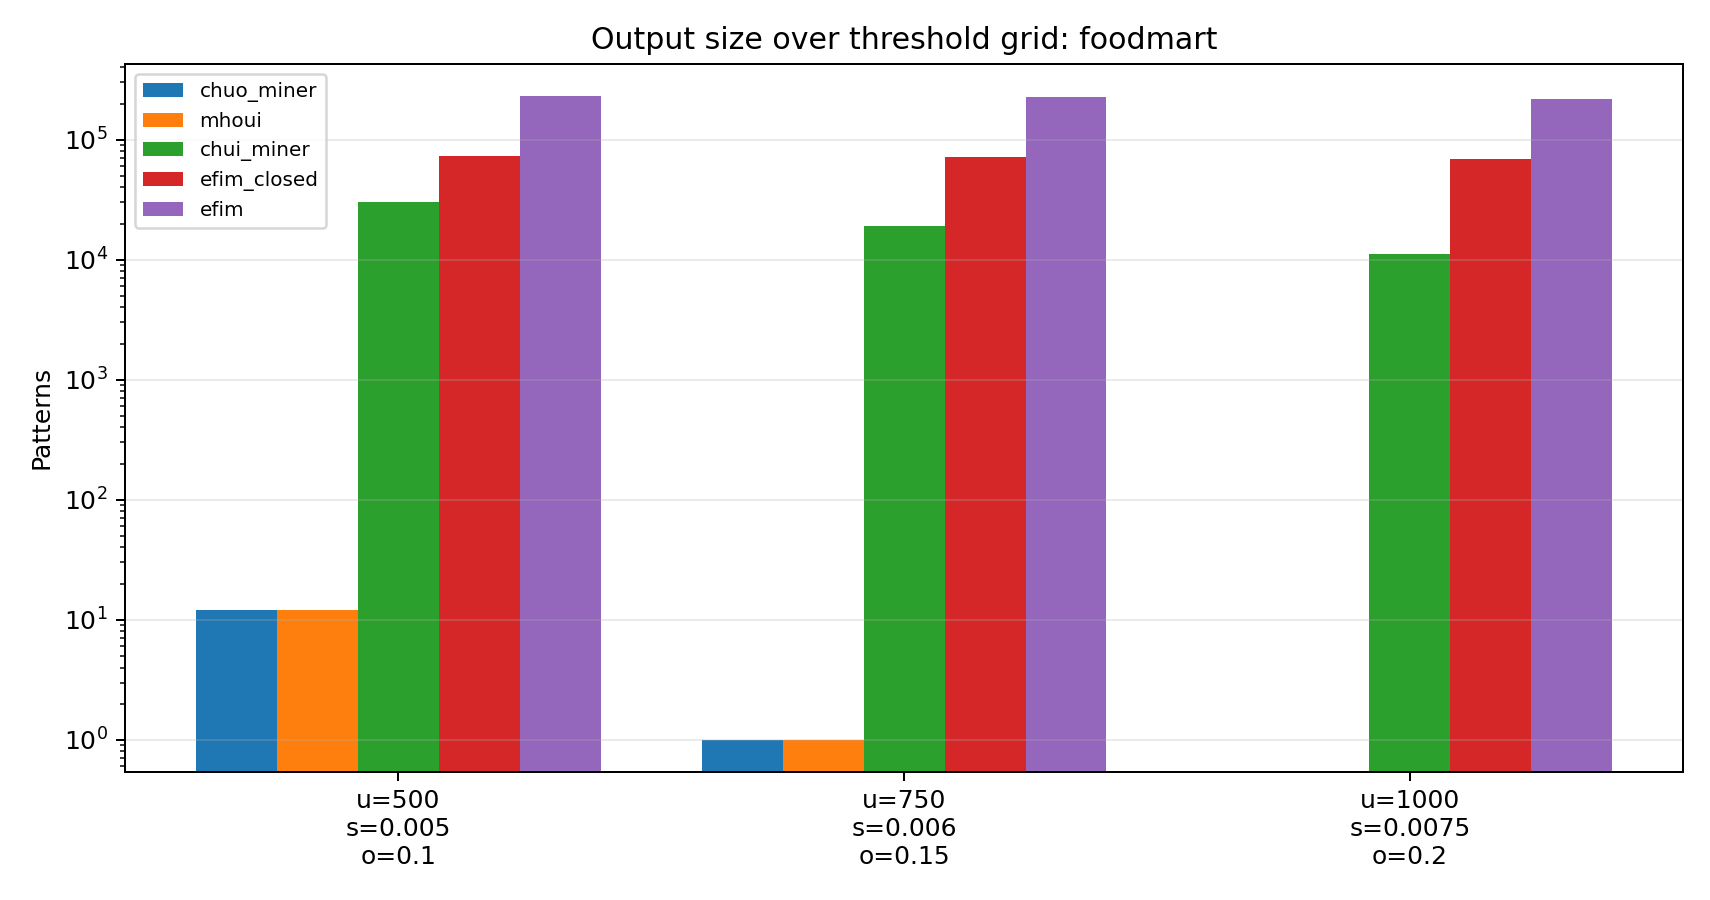
\includegraphics[width=\linewidth]{../results/chuo_q1_grid/foodmart_output_count_grid.png}
    \caption{Foodmart}
\end{subfigure}
\hfill
\begin{subfigure}{0.32\textwidth}
    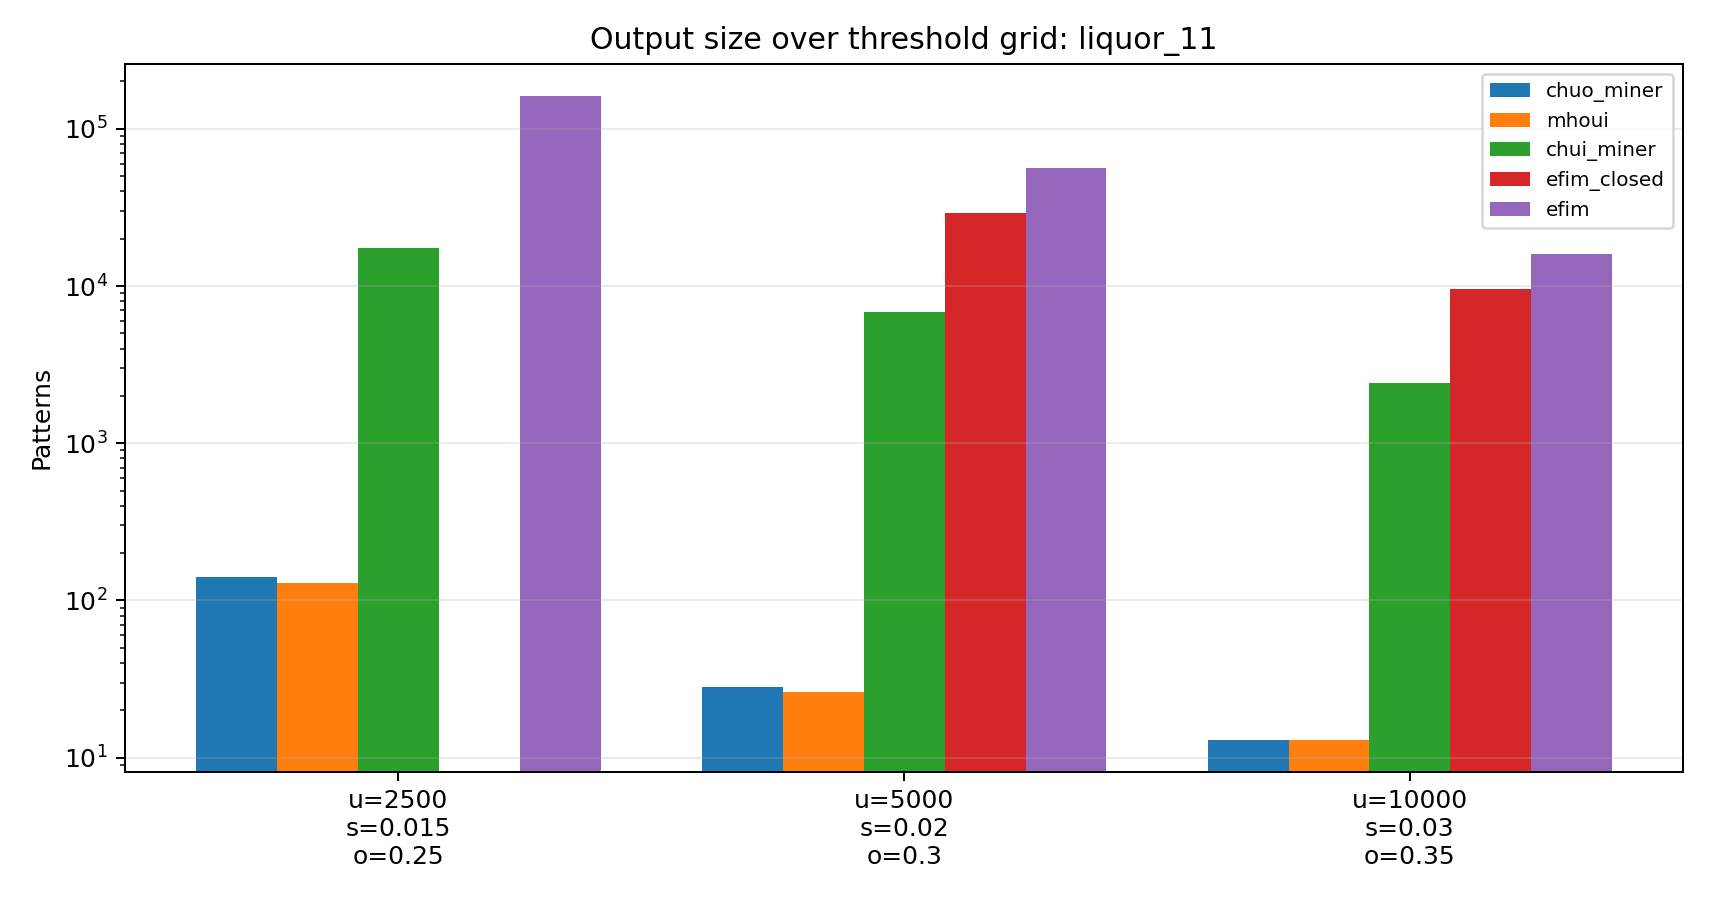
\includegraphics[width=\linewidth]{../results/chuo_q1_grid/liquor_11_output_count_grid.png}
    \caption{Liquor\_11}
\end{subfigure}
\hfill
\begin{subfigure}{0.32\textwidth}
    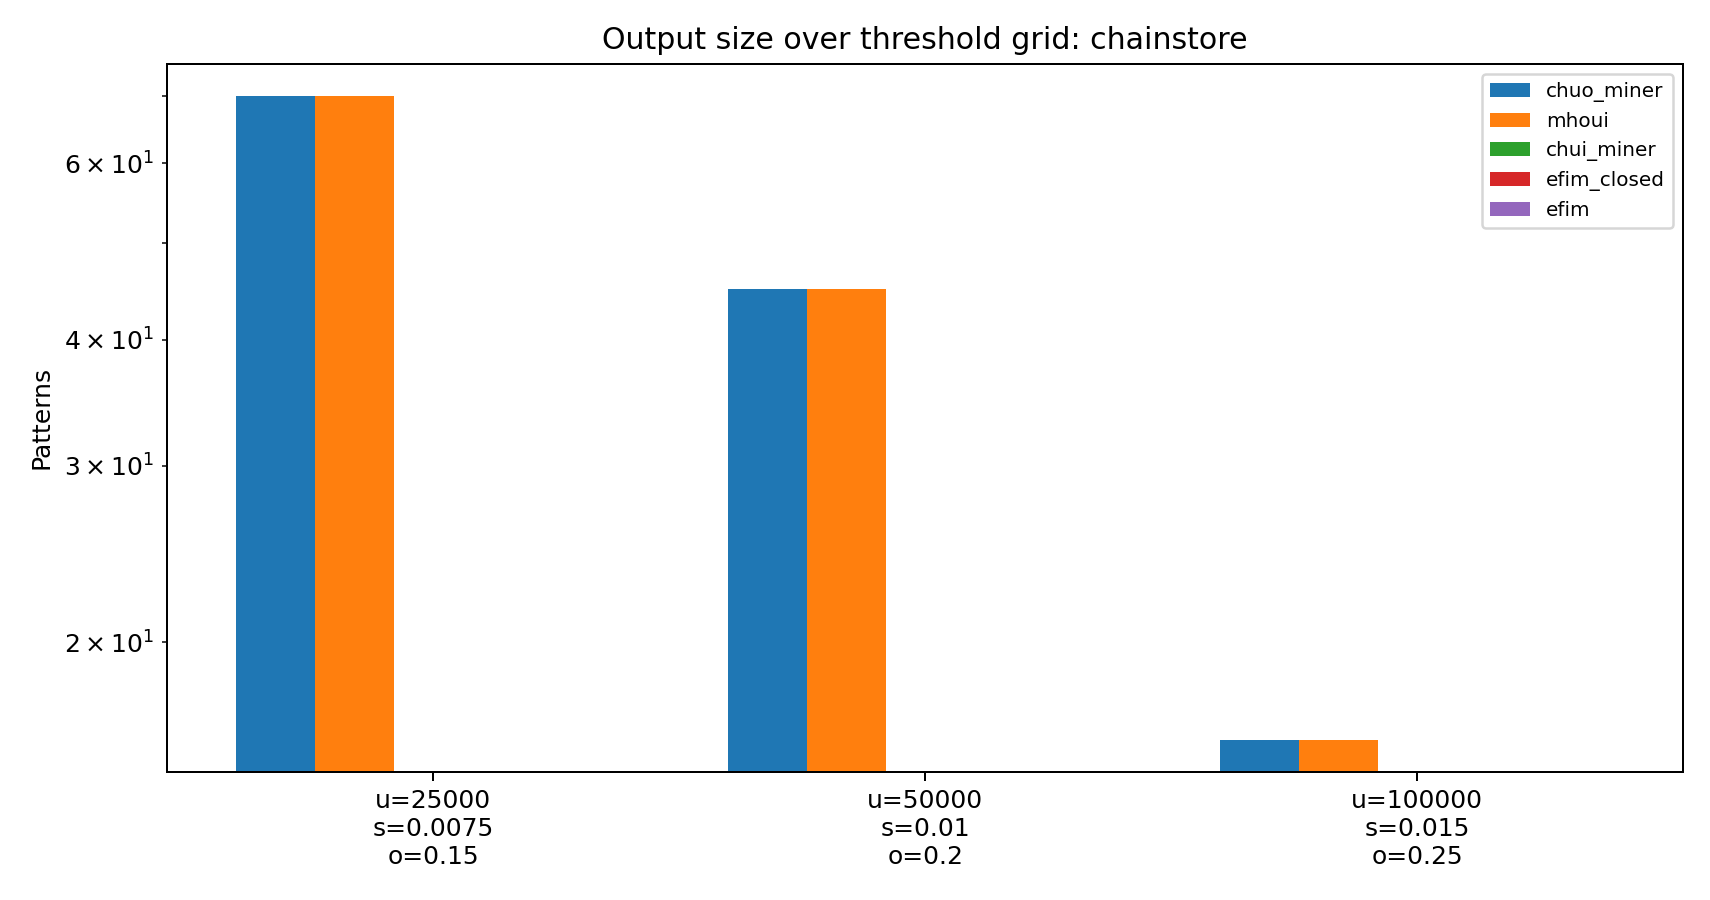
\includegraphics[width=\linewidth]{../results/chuo_q1_grid/chainstore_output_count_grid.png}
    \caption{Chainstore}
\end{subfigure}
\caption{Output size comparison over threshold grids. The y-axis is logarithmic in the generated plots.}
\label{fig:output}
\end{figure}

\subsection{Runtime and Scalability}

MHOUI is the fastest hybrid baseline because it does not compute support closures or CHUO-signatures. CHUO-Miner is slower than MHOUI, but it solves the stricter closed hybrid task. Against CHUI-Miner, EFIM-Closed, and EFIM, CHUO-Miner is substantially more scalable on the hybrid task. On Chainstore, CHUO-Miner completes in 3.32, 3.01, and 2.36 seconds across the three settings, while all three utility-only or closed-utility baselines timeout.

\begin{table}[H]
\centering
\caption{Runtime in seconds over diverse thresholds.}
\label{tab:runtime}
\small
\begin{adjustbox}{max width=\textwidth}
\begin{tabular}{llrrrrr}
\toprule
Dataset & Setting & CHUO & MHOUI & CHUI & EFIM-Closed & EFIM \\
\midrule
\multirow{3}{*}{Foodmart}
& relaxed & 0.003 & 0.002 & 2.944 & 0.199 & 0.235 \\
& medium & 0.001 & 0.001 & 2.600 & 0.224 & 0.243 \\
& strict & 0.001 & 0.001 & 1.910 & 0.290 & 0.362 \\
\midrule
\multirow{3}{*}{Liquor\_11}
& relaxed & 2.000 & 0.168 & 28.761 & TO & 53.187 \\
& medium & 2.274 & 0.154 & 14.848 & 46.107 & 21.202 \\
& strict & 1.666 & 0.108 & 6.101 & 15.872 & 9.750 \\
\midrule
\multirow{3}{*}{Chainstore}
& relaxed & 3.316 & 0.965 & TO & TO & TO \\
& medium & 3.006 & 0.792 & TO & TO & TO \\
& strict & 2.356 & 0.819 & TO & TO & TO \\
\bottomrule
\end{tabular}
\end{adjustbox}
\end{table}

\begin{figure}[H]
\centering
\begin{subfigure}{0.32\textwidth}
    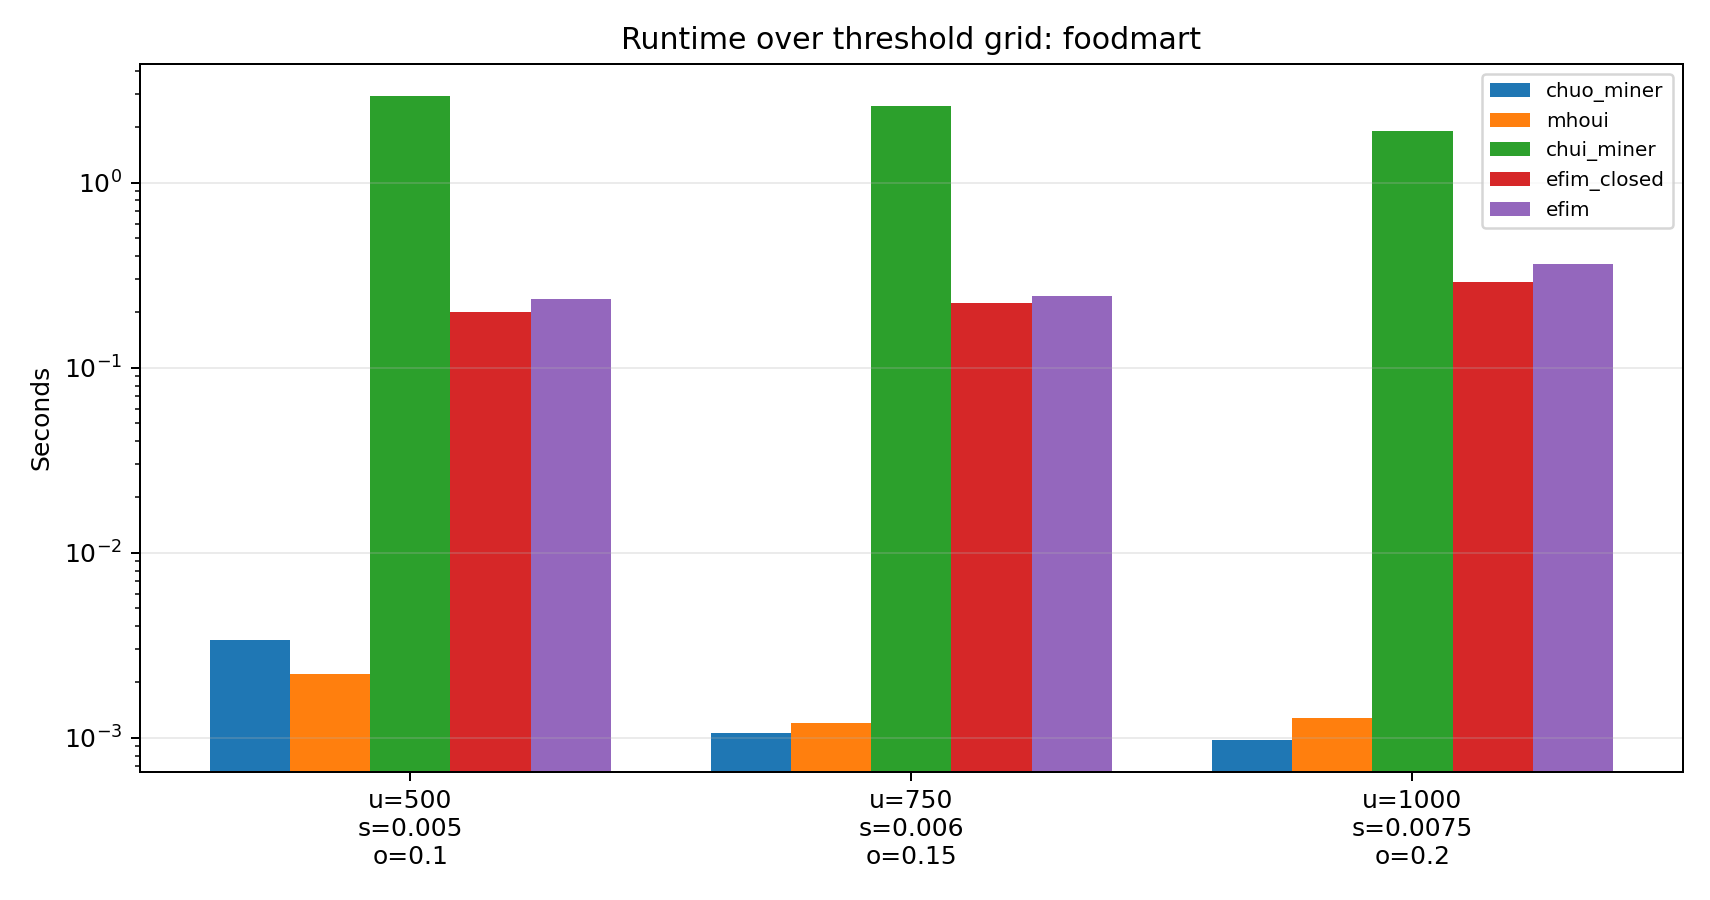
\includegraphics[width=\linewidth]{../results/chuo_q1_grid/foodmart_runtime_sec_grid.png}
    \caption{Foodmart}
\end{subfigure}
\hfill
\begin{subfigure}{0.32\textwidth}
    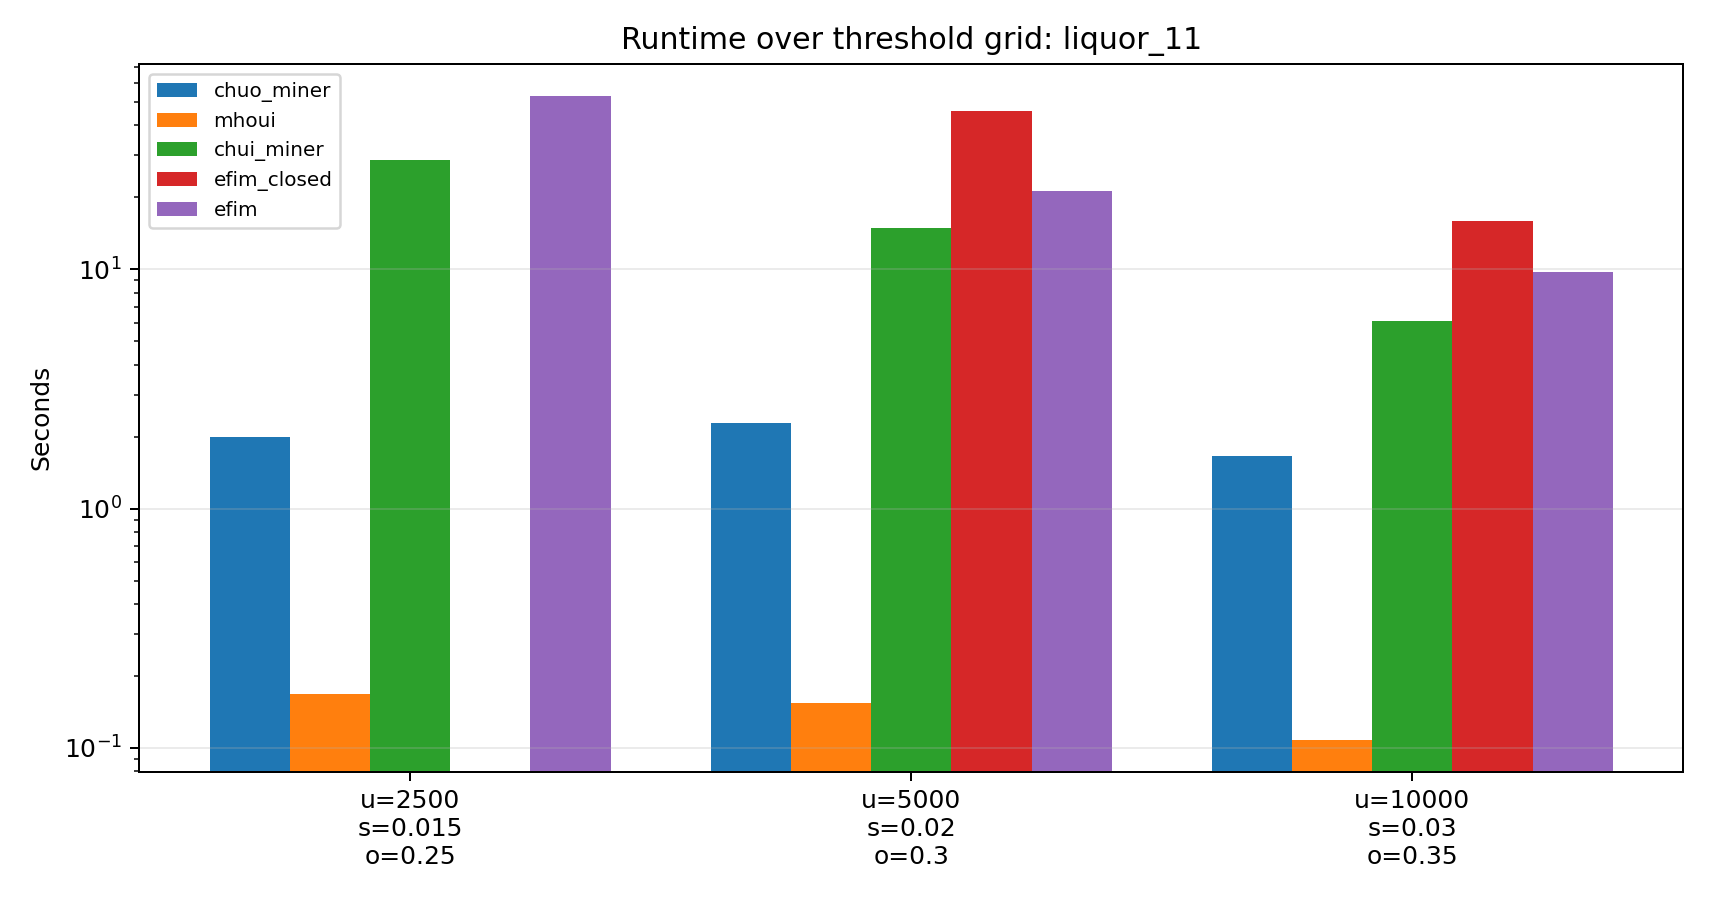
\includegraphics[width=\linewidth]{../results/chuo_q1_grid/liquor_11_runtime_sec_grid.png}
    \caption{Liquor\_11}
\end{subfigure}
\hfill
\begin{subfigure}{0.32\textwidth}
    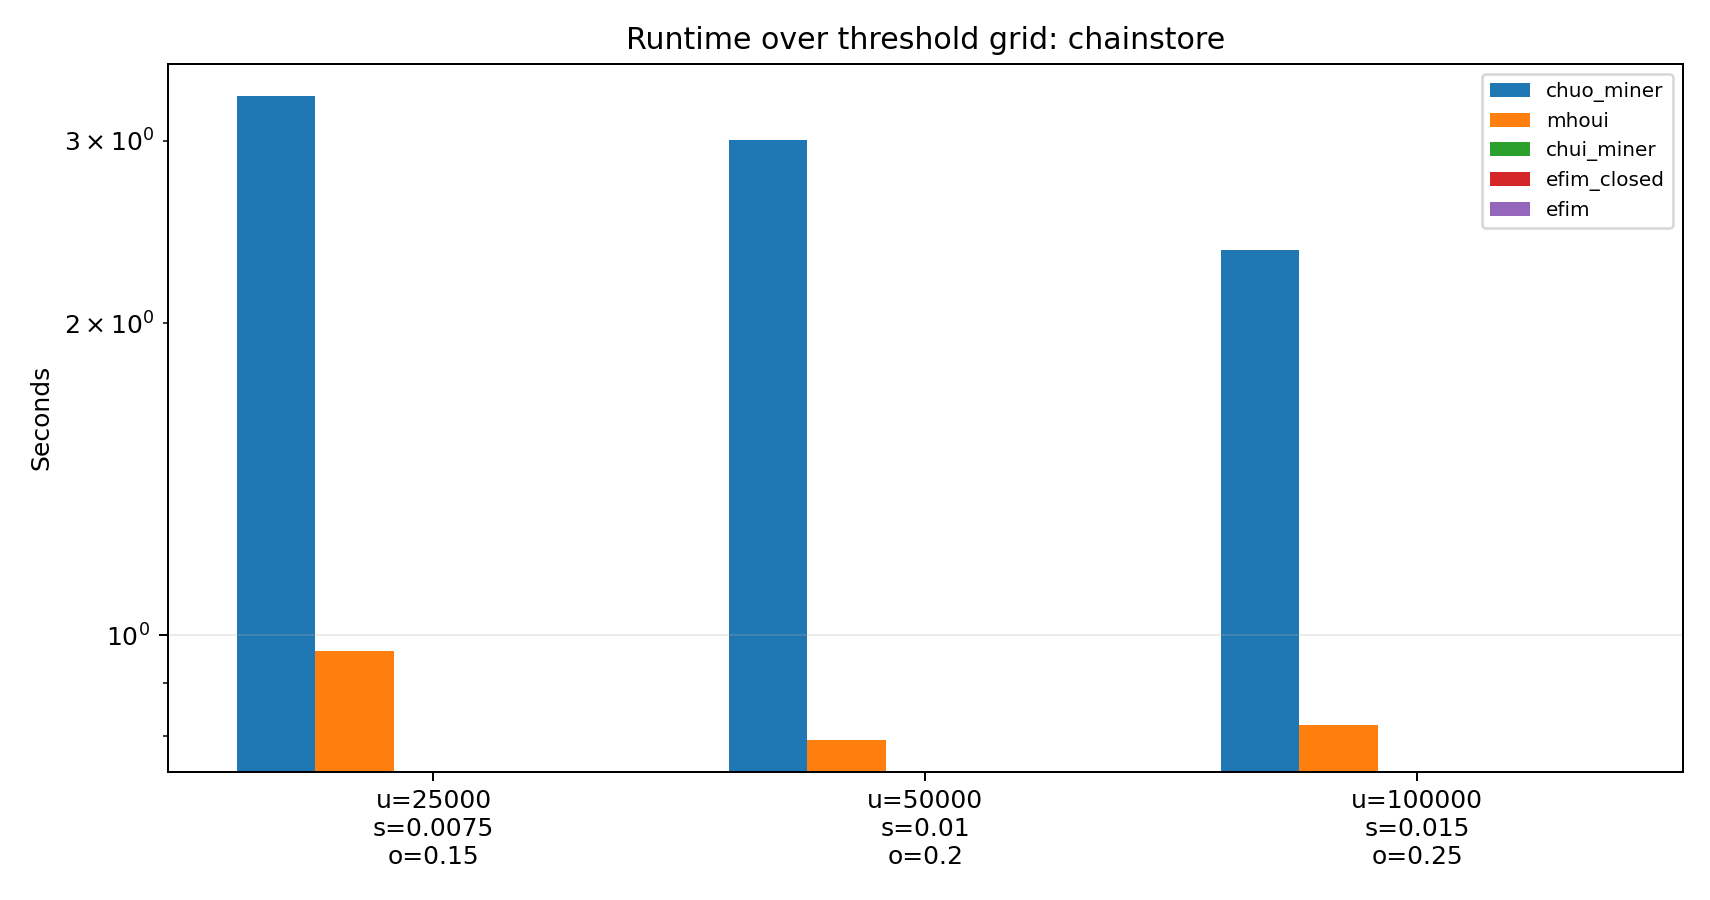
\includegraphics[width=\linewidth]{../results/chuo_q1_grid/chainstore_runtime_sec_grid.png}
    \caption{Chainstore}
\end{subfigure}
\caption{Runtime comparison over threshold grids.}
\label{fig:runtime}
\end{figure}

\subsection{Memory and Result Footprint}

CHUO-Miner requires more memory than MHOUI on Chainstore because it stores singleton bitsets and closure metadata. However, its result footprint is still compact and reconstructable. Compared with EFIM and closed-utility baselines, CHUO-Miner avoids large result sets. On Foodmart at the relaxed setting, CHUO-Miner's estimated result disk footprint is 1,824 bytes, compared with 243,832 bytes for CHUI-Miner, 589,272 bytes for EFIM-Closed, and 6,690,487 bytes for EFIM.

\begin{figure}[H]
\centering
\begin{subfigure}{0.32\textwidth}
    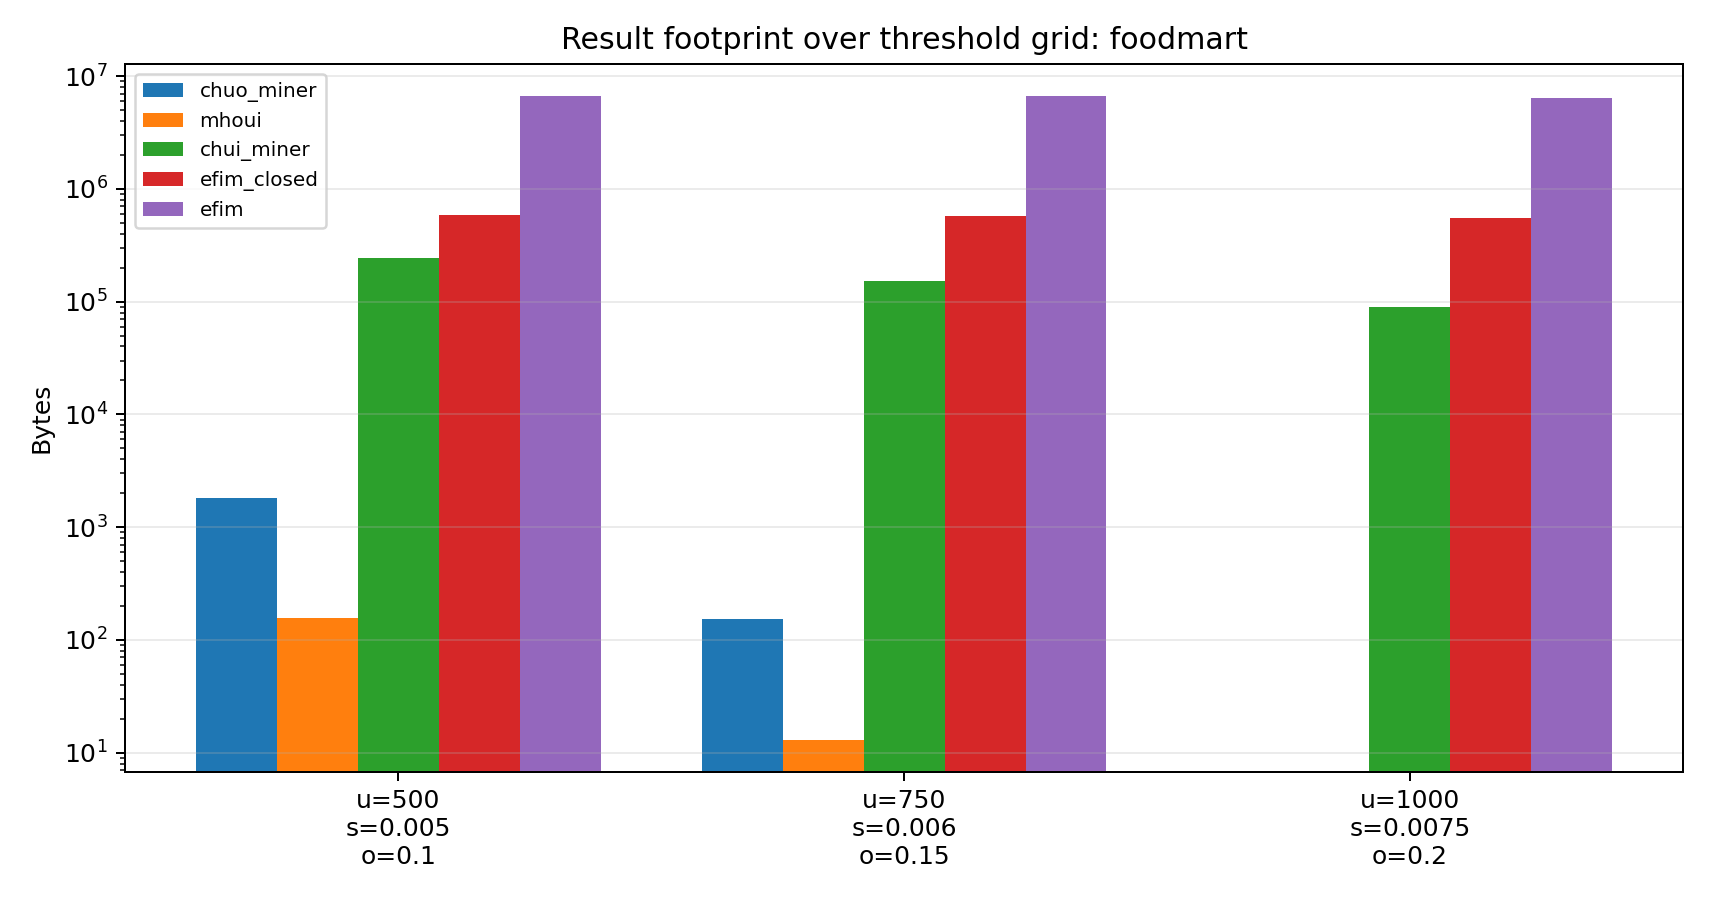
\includegraphics[width=\linewidth]{../results/chuo_q1_grid/foodmart_result_disk_est_bytes_grid.png}
    \caption{Foodmart}
\end{subfigure}
\hfill
\begin{subfigure}{0.32\textwidth}
    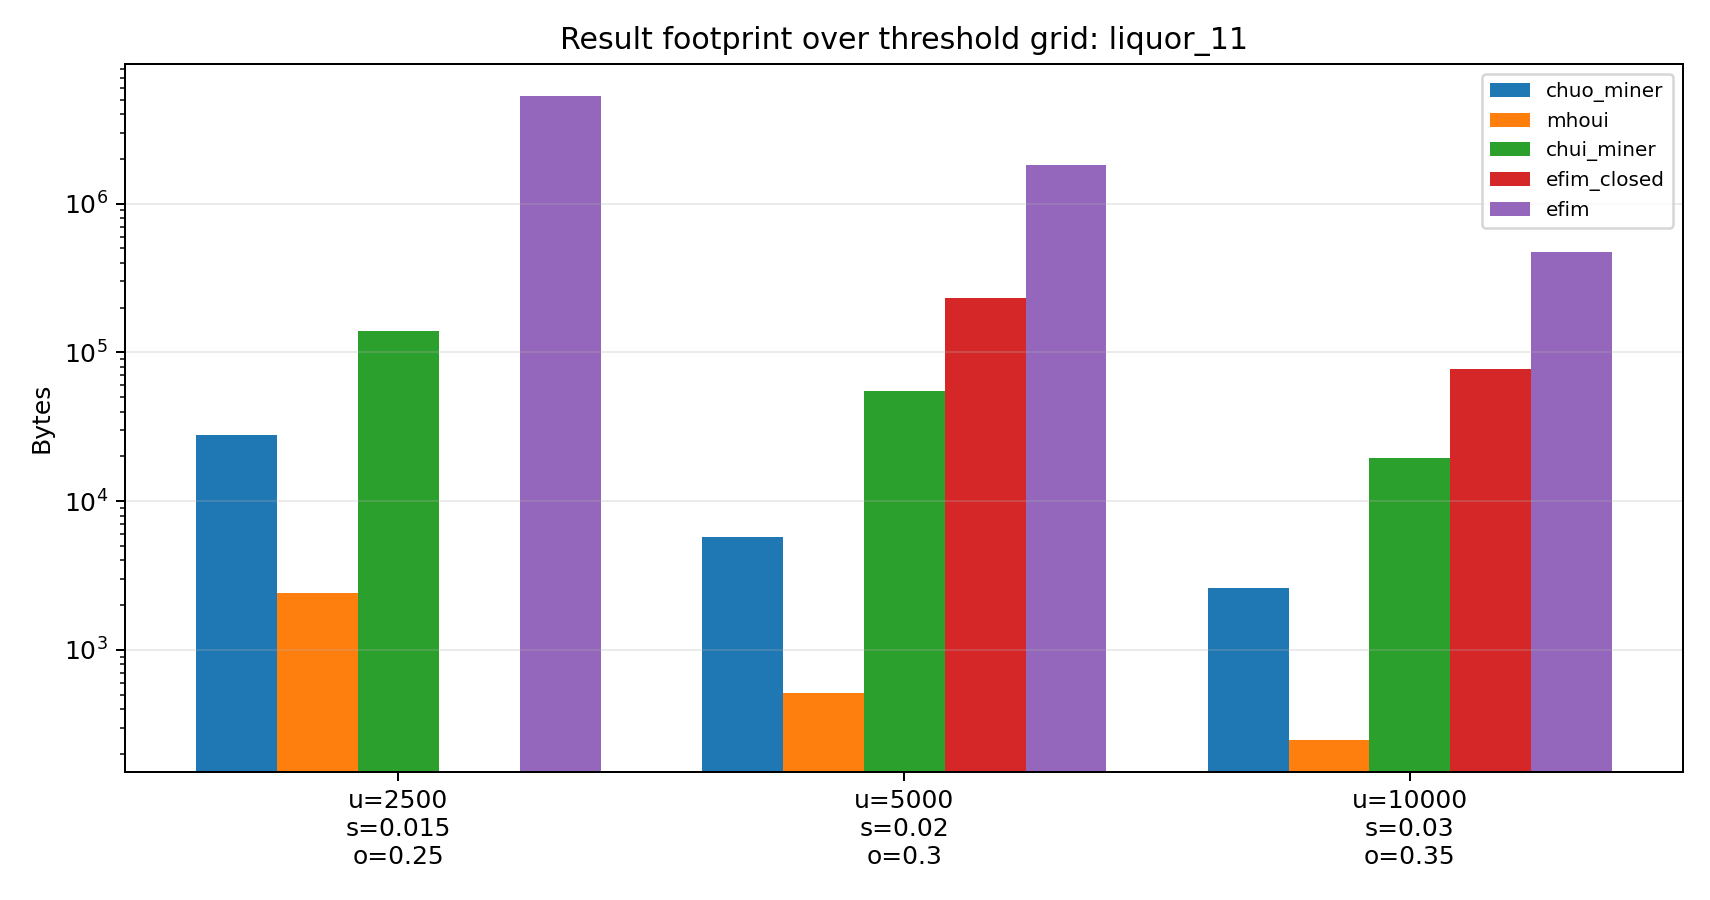
\includegraphics[width=\linewidth]{../results/chuo_q1_grid/liquor_11_result_disk_est_bytes_grid.png}
    \caption{Liquor\_11}
\end{subfigure}
\hfill
\begin{subfigure}{0.32\textwidth}
    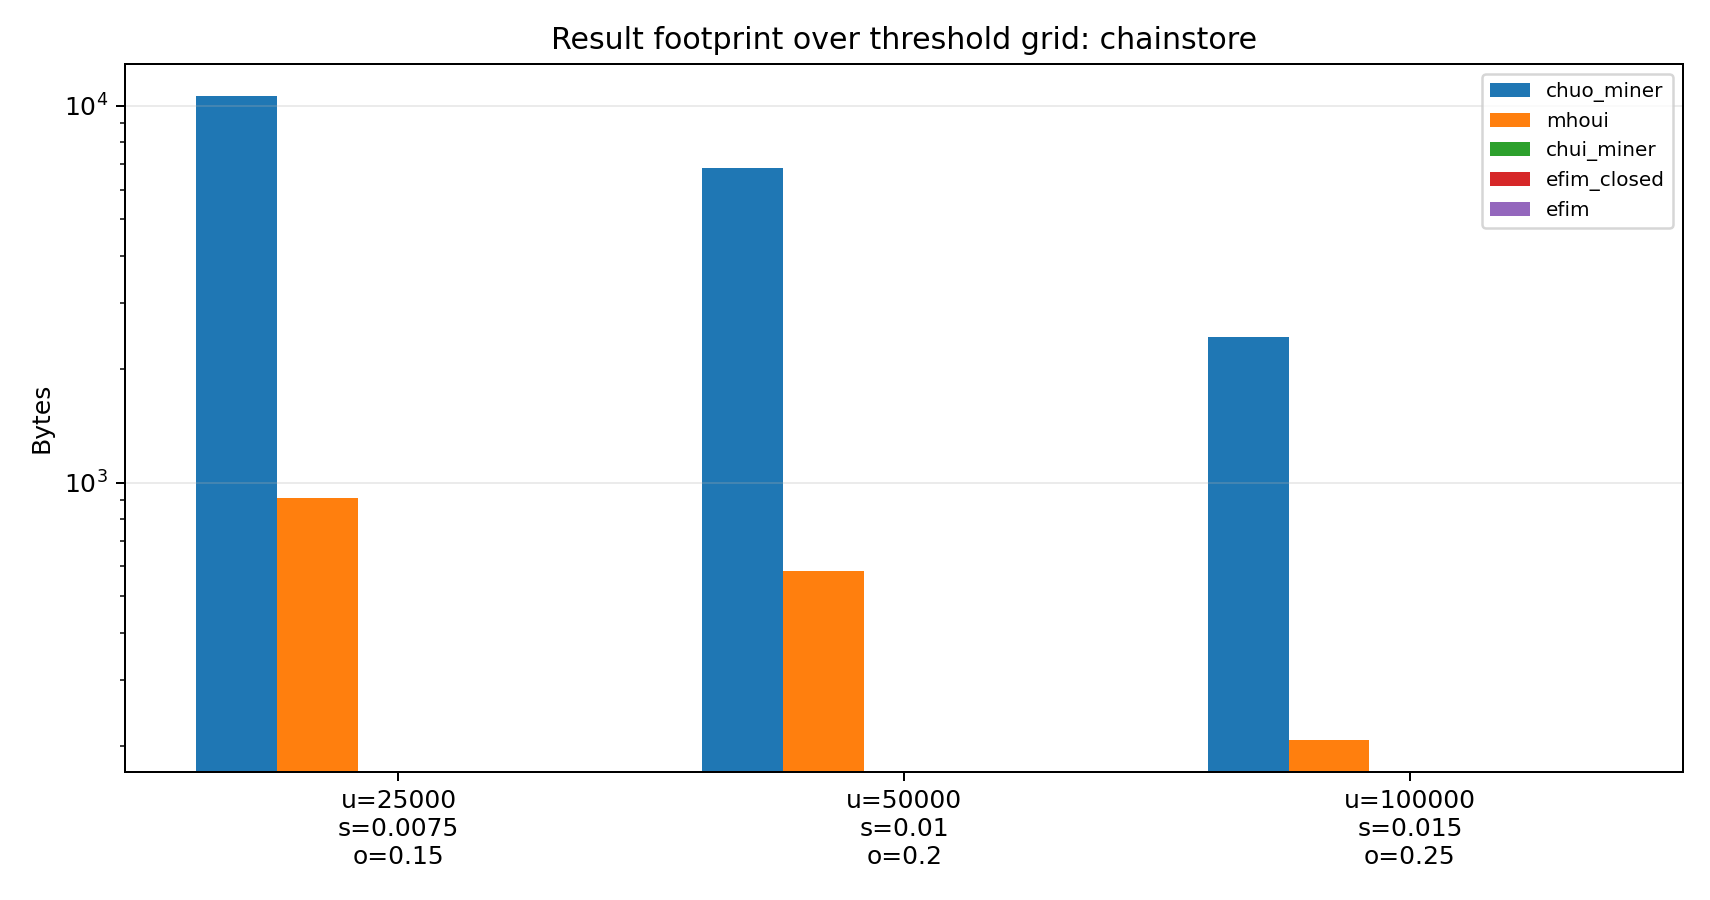
\includegraphics[width=\linewidth]{../results/chuo_q1_grid/chainstore_result_disk_est_bytes_grid.png}
    \caption{Chainstore}
\end{subfigure}
\caption{Estimated output footprint. CHUO-Miner stores closed hybrid signatures rather than all raw HUIs.}
\label{fig:footprint}
\end{figure}

\subsection{Interpretation}

The results show that CHUO-Miner is not simply a faster MHOUI variant. MHOUI wins on raw runtime because it does not enforce support-closure or build lossless CHUO-signatures. CHUO-Miner's advantage is representational: it returns support-closed high-utility occupancy representatives and can reconstruct support-equivalent redundant subpatterns through \(V_C(i)\) and \(R_C\). This makes CHUO-Miner better suited for compact, interpretable, lossless hybrid pattern mining.

Against EFIM, CHUI-Miner, and EFIM-Closed, CHUO-Miner is clearly stronger for the proposed task. These baselines either ignore occupancy, ignore closure, or both. Their output sizes are much larger, and on Chainstore they fail to finish under the timeout while CHUO-Miner completes all threshold settings.

\section{Threats to Validity}

The first threat is that MHOUI solves a nearby but different problem. It is the closest hybrid baseline, but it does not provide support-closed representatives or CHUO-signatures. The second threat is that CHUI-Miner, EFIM-Closed, and EFIM do not enforce occupancy; they are included to show how classical utility and closed-utility outputs behave when used as parent-family baselines. The third threat is threshold sensitivity, addressed here by evaluating three settings per dataset. The fourth threat is timeout selection; a longer timeout could produce additional baseline results on Chainstore, but the observed timeouts still indicate poor scalability under the tested setting.

\section{Conclusion}

This paper introduced CHUOIM and CHUO-Miner, a closed high-utility occupancy mining framework based on support closure, absolute utility, classical average occupancy, and lossless CHUO-signatures. The theoretical result is that closure is the Pareto-maximum representative of each support-equivalence class for both utility and classical occupancy under positive utilities. The algorithmic result is a vertical COU-list miner with RUU pruning, OUB pruning, backward closure pruning, forward closure jumping, and closure hashing.

The diverse threshold-grid experiments show that CHUO-Miner produces compact closed hybrid representatives, scales on Chainstore where EFIM, EFIM-Closed, and CHUI-Miner timeout, and offers stronger semantics than MHOUI at the cost of slower runtime. The honest conclusion is therefore precise: MHOUI is faster, but CHUO-Miner is the stronger closed, compact, lossless hybrid representation.

\begin{thebibliography}{99}

\bibitem{Liu2005TwoPhase}
Ying Liu, Wei-keng Liao, and Alok Choudhary.
\newblock A two-phase algorithm for fast discovery of high utility itemsets.
\newblock In \emph{Proceedings of PAKDD}, pages 689--695, 2005.

\bibitem{Liu2012HUIMiner}
Mengchi Liu and Junfeng Qu.
\newblock Mining high utility itemsets without candidate generation.
\newblock In \emph{Proceedings of CIKM}, pages 55--64, 2012.

\bibitem{FournierViger2014FHM}
Philippe Fournier-Viger, Cheng-Wei Wu, Souleymane Zida, and Vincent S. Tseng.
\newblock FHM: Faster high-utility itemset mining using estimated utility co-occurrence pruning.
\newblock In \emph{Proceedings of ISMIS}, pages 83--92, 2014.

\bibitem{Zida2017EFIM}
Souleymane Zida, Philippe Fournier-Viger, Jerry Chun-Wei Lin, Cheng-Wei Wu, and Vincent S. Tseng.
\newblock EFIM: A fast and memory efficient algorithm for high-utility itemset mining.
\newblock \emph{Knowledge and Information Systems}, 51:595--625, 2017.

\bibitem{Wu2015CHUIMiner}
Cheng-Wei Wu, Philippe Fournier-Viger, Philip S. Yu, and Vincent S. Tseng.
\newblock Mining closed high utility itemsets without candidate generation.
\newblock In \emph{Proceedings of IEEE SMC}, pages 199--204, 2015.

\bibitem{Deng2020HOI}
Zhi-Hong Deng.
\newblock Mining high occupancy itemsets.
\newblock \emph{Future Generation Computer Systems}, 102:222--229, 2020.

\bibitem{Gan2020HUOPM}
Wensheng Gan, Jerry Chun-Wei Lin, Philippe Fournier-Viger, Han-Chieh Chao, and Philip S. Yu.
\newblock HUOPM: High-utility occupancy pattern mining.
\newblock \emph{IEEE Transactions on Cybernetics}, 50(3):1195--1208, 2020.

\end{thebibliography}

\end{document}
